\clearpage

\begin{center}
  {\color{accent}\large PART 4}\par
  \vspace{0.25em}
  {\Large\bfseries Decision Tree 小實作}\par
\end{center}

\vspace{1.0em}

\section*{1. Experimental Setup}
\sectionrule

為了和 Part 2 公平比較，我直接依 \dataterm{results/train\_test\_split.csv} 重建相同的 stratified split：training set 273 筆、test set 69 筆，並沿用 culmen length、culmen depth、flipper length 與 body mass 四個 numerical features。\dataterm{source\_row} 只負責追蹤資料來源，沒有放入模型。

主模型使用 Decision Tree classifier。我將 criterion 設為 Gini impurity、maximum depth 設為 3，random state 則固定為 42。Decision Tree 每次只用一個 feature 的 threshold 切分資料，不會像 distance-based KNN 一樣，讓數值範圍較大的 body mass 自動取得較大權重。因此主模型保留原始單位，不另外做 scaling，圖上的 threshold 也能直接用實際單位解讀。

\section*{2. Tree Structure and Root Split}
\sectionrule

\begin{figure}[H]
\centering
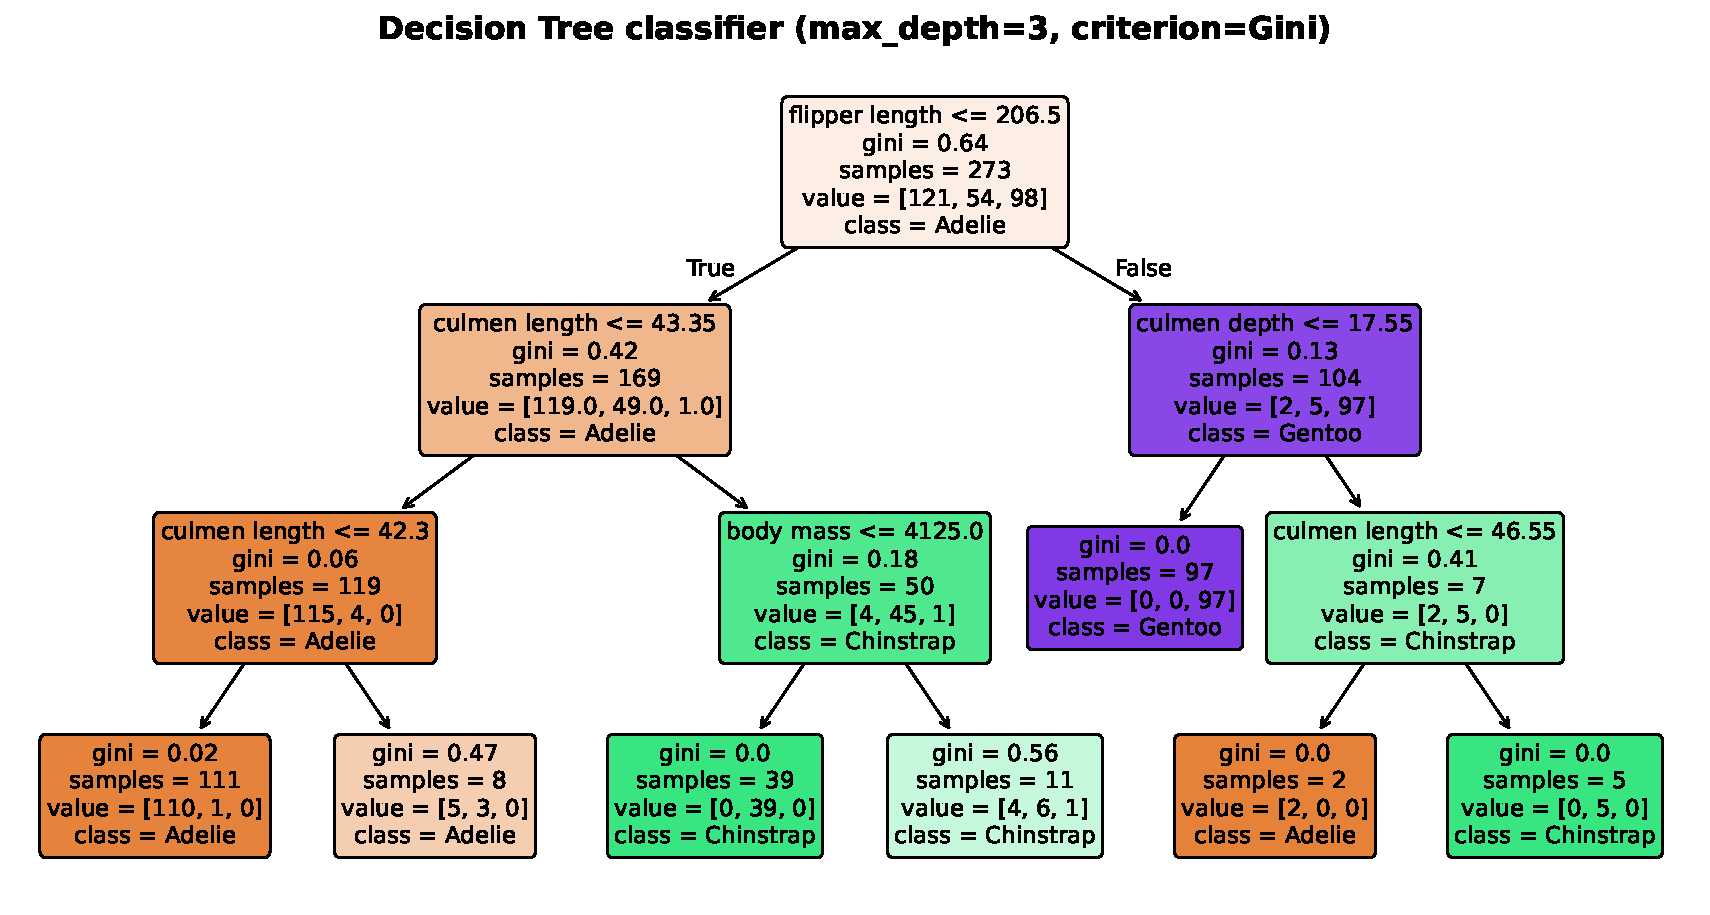
\includegraphics[width=\linewidth]{part4_decision_tree.pdf}
\caption{Decision Tree 主模型。每個節點顯示 split 條件、Gini、samples、各類別筆數與預測 class。}
\end{figure}

這棵樹的實際深度為 3，共有 13 個 nodes 與 7 個 leaves。第一個條件，也就是 root node，使用 \dataterm{flipper\_length\_mm}，threshold 為 206.5 mm：小於等於 206.5 mm 的企鵝走左支，較大的走右支。這個 split 先把多數 Gentoo 和另外兩個物種分開，後面再用 culmen length、culmen depth 與 body mass 繼續細分。

Gini 越低，代表節點裡的 class 越單純。建樹時，模型會尋找能讓子節點加權 Gini 降得最多的候選 split。因此 root 看重的是哪個條件最能分開 training data 中的 species，feature 本身的數值範圍並不會讓它優先被選中。

\section*{3. Manual Prediction Path}
\sectionrule

我從 test set 中挑出 \dataterm{source\_row=3} 的企鵝，手動走一次 prediction path。它的 actual class 是 Adelie，features 如下：

\begin{table}[H]
\centering
\small
\begin{tabular}{lrrrr}
\toprule
 & \textbf{Culmen length} & \textbf{Culmen depth} & \textbf{Flipper length} & \textbf{Body mass} \\
\midrule
Feature value & 39.5 mm & 17.4 mm & 186 mm & 3800 g \\
\bottomrule
\end{tabular}
\end{table}

從 root 開始依序判斷：

\begin{enumerate}[leftmargin=1.8em,itemsep=0.35em]
  \item $\dataterm{flipper\_length\_mm}=186 \leq 206.5$，走左支。
  \item $\dataterm{culmen\_length\_mm}=39.5 \leq 43.35$，再走左支。
  \item $\dataterm{culmen\_length\_mm}=39.5 \leq 42.30$，到達 leaf node 3。
\end{enumerate}

最後到達的 leaf 預測 class 為 Adelie，因此模型的預測和 actual class 相同。從這條 prediction path 也能直接看出，Decision Tree 處理一筆資料時，只需要依序檢查 root 到 leaf 之間的幾個 threshold，整個判斷過程很容易追蹤。

\clearpage
\section*{4. Test-set Performance}
\sectionrule

\begin{figure}[H]
\centering
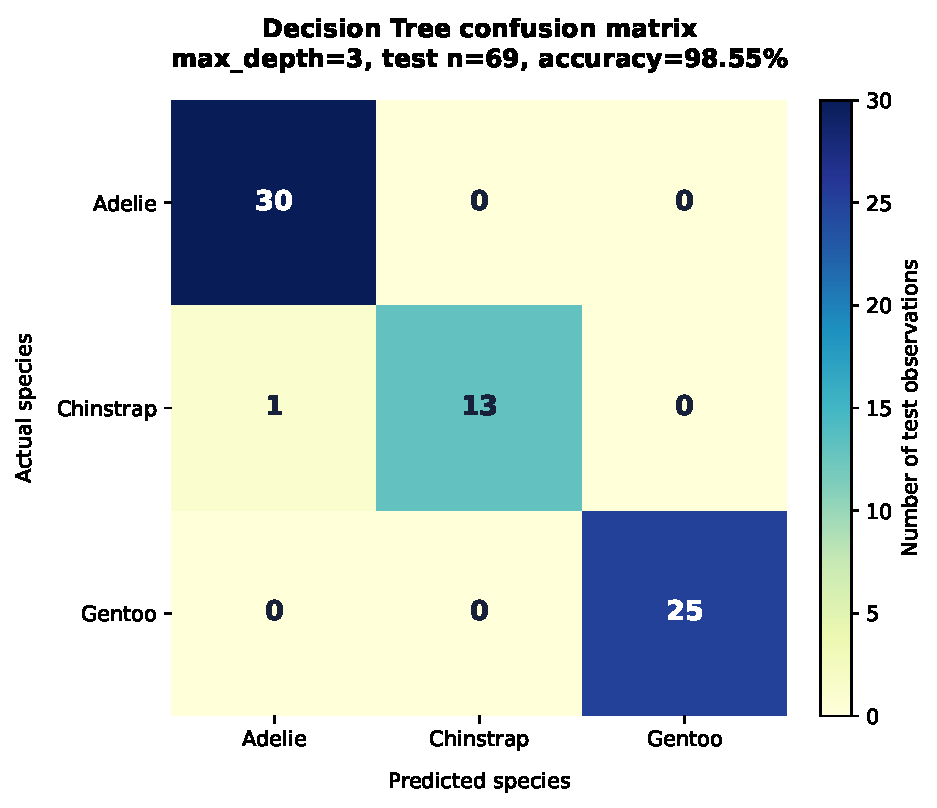
\includegraphics[width=0.69\linewidth]{part4_decision_tree_confusion_matrix.pdf}
\caption{Decision Tree 主模型在固定 test set 的 confusion matrix。列為 actual class，欄為 predicted class。}
\end{figure}

主模型在 69 筆 test data 中判對 68 筆，accuracy 為
\[
\frac{68}{69}=98.55\%,
\qquad
\text{error rate}=1-\frac{68}{69}=\frac{1}{69}=1.45\%.
\]
從 confusion matrix 來看，Adelie 的 30 筆和 Gentoo 的 25 筆全部判對；14 筆 Chinstrap 中則有 13 筆判對，剩下 1 筆被判成 Adelie。唯一的錯誤落在 Adelie 與 Chinstrap 之間，Gentoo 沒有和其他物種混淆。

\section*{5. Small Comparison: Maximum Depth}
\sectionrule

這裡我只調整 maximum depth，其餘資料、criterion 與 random state 都維持不變：

\begin{table}[H]
\centering
\small
\begin{tabularx}{\linewidth}{lrrrrY}
\toprule
\textbf{設定} & \textbf{實際深度} & \textbf{Nodes} & \textbf{Leaves} & \textbf{Accuracy} & \textbf{Test errors} \\
\midrule
$\dataterm{max\_depth}=3$ & 3 & 13 & 7 & 98.55\% & 1 Chinstrap $\rightarrow$ Adelie \\
$\dataterm{max\_depth}=2$ & 2 & 7 & 4 & 98.55\% & 1 Chinstrap $\rightarrow$ Adelie \\
\bottomrule
\end{tabularx}
\end{table}

深度 2 的樹少了 6 個 nodes 與 3 個 leaves，在這組 test set 上卻得到完全相同的 predictions。換句話說，第三層雖然讓 training data 分得更細，對這 69 筆 test data 並沒有帶來實際改善。若只看這次的泛化表現，我會偏向較精簡的深度 2；主模型仍保留作業建議的深度 3，因為它能展示更完整、同時仍然可讀的 tree structure。
